% !TEX root=../main.tex

\section{Examples}
\label{sec:examples}

In this section we study three examples to illustrate how the language \TOPHAT works and what kind of properties we would like to prove.



\subsection{Positive value}

This example demonstrates how to prove that a program only accepts positive values as inputs.
Consider the program in \cref{lst:abs}.

\begin{TASK}[float=h
            ,caption=A task that only accepts positive values as inputs.
            ,label=lst:abs
            ]
  enter Int >>= \ x. if x > 0 then edit x else fail
\end{TASK}

It asks the user to input a value of type $\Int$.
This value is then passed on to the right hand side.
If the value is greater than zero, an editor containing the entered value is returned.
Otherwise the step does not proceed and the user has to enter a different value.

Imagine that we would like to prove that no matter which value is given as input,
the only possible outcome is a value greater than zero.

Symbolic execution of this program proceeds as follows.
The symbolic execution engine generates a fresh symbolic input $s$ for the editor on the left.
The engine then arrives at the conditional.
In order to take the then-branch, the condition $s > 0$ needs to hold.
This branch will then result in $\Edit s$, in which case the program has an observable value.
The engine records this endpoint together with its path condition $s > 0$.
The else-branch applies if the condition does not hold, but this leads to a failing task.
Therefore, the step is not taken and the programs stays the same.
No additional program state is generated.

Symbolic execution returns a list of all possible program end states, together with the path conditions that led to them.
If all end states agree with the desired property, it is guaranteed that the property holds for all possible inputs.

In this example, the only end state is the expression $\Edit s$ with path condition $s > 0$.
From that we can conclude that no matter what input is given, the only result value possible has to be greater than zero.



\subsection{Tax subsidy request}

\citet{conf/sfp/StutterheimAP17} worked with the Dutch tax office to develop a demonstrator for a fictional but realistic law about solar panel subsidies.
In this section we study a simplified version of this, translated to \TOPHAT, to illustrate how symbolic execution can be used to prove that the program implements the law.

This example proves that a citizen will get subsidy only under the following conditions.
\begin{itemize}
\item The roofing company has confirmed that they installed solar panels for the citizen.
\item The tax officer has approved the request.
\item The tax officer can only approve the request if the roofing company has confirmed, and the request is filed within one year of the invoice date.
\item The amount of the granted subsidy is maximal 600 EUR.
\end{itemize}

\lstset{emph={invoiceDate,today,confirmed,invoiceAmount,approved}}
\begin{TASK}[float=ht
            ,numbers=right
            ,caption=Subsidy request and approval workflow at the Dutch tax office.
            ,label=lst:tax
            ]
  let provideCitizenInformation = enter Date in
  let provideDocuments = enter Amount <&> enter Date in
  let companyConfirm = edit True <?> edit False in
  let officerApprove = \ invoiceDate. \ today. \ confirmed.
    edit False <?> if (today - invoiceDate < 365 /\ confirmed) |\label{lst:tax:officer-approve-def}|
      then edit True
      else fail in
  provideCitizenInformation >>= \ today.|\label{lst:tax:citizen-info}|
  provideDocuments <&> companyConfirm >>= |\label{lst:tax:documents-and-company-confirm}|
    \ <<<<invoiceAmount, invoiceDate>>, confirmed>>.
  officerApprove invoiceDate today confirmed >>= \ approved.|\label{lst:tax:officer-approve}|
  let subsidyAmount = if approved
    then min 600 (invoiceAmount / 10) else 0 in
  edit <<subsidyAmount, approved, confirmed, invoiceDate, today>>|\label{lst:tax:result}|
\end{TASK}

\begin{figure}[ht]
  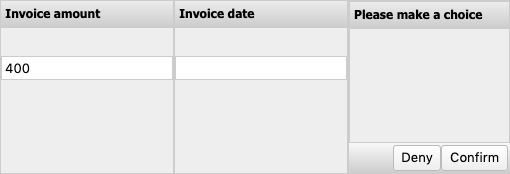
\includegraphics[width=\columnwidth]{figures/tax-enter}
  \caption{
    Graphical user interface for the task in \cref{lst:tax}.
    In parallel, the citizen is asked to enter the invoice amount and the invoice date of the installed solar panels,
    and the roofing company is asked to deny or confirm they actually installed the solar panels.
  }
  \label{fig:tax}
\end{figure}

\Cref{lst:tax} shows the program.
To enhance readability of the example,
we omit type annotations and make use of pattern matching on tuples.
The program works as follows.
First, the citizen has to enter their personal information (\cref{lst:tax:citizen-info}).
In the original demonstrator this included the citizen service number, name, and home address.
Here, we simplified the example so that the citizen only has to enter the invoice date.
A date is specified using an integer representing the number of days since 1 January 2000.

In the next step (\cref{lst:tax:documents-and-company-confirm}), in parallel the citizen has to provide the invoice documents of the installed solar panels, while the roofing company has to confirm that they have actually installed solar panels at the citizen's address.
Once the invoice and the confirmation are there, the tax officer has to approve the request (\cref{lst:tax:officer-approve}).
The officer can always decline the request, but they can only approve it if the roofing company has confirmed and the application date is within one year of the invoice date (\cref{lst:tax:officer-approve-def}).
The result of the program is the amount of the subsidy, together with all information needed to prove the required properties (\cref{lst:tax:result}).
The graphical user interface belonging to two steps in this process are shown in \cref{fig:tax}.

The result of the overall task is a tuple with the subsidy amount, the officer's approval, the roofing company's confirmation, the invoice amount, the invoice date, and today's date.
Returning all this information allows the following predicate to be stated, which verifies the correctness of the implementation.
The predicate has 5 free variables, which correspond to the returned values.
\setcounter{equation}{0}
\begin{align}
\psi(s,a,c,i,t)
   & =      s \geq 0 \implies c \label{for:tax:psi-confirmed}
\\ & \wedge s \geq 0 \implies a \label{for:tax:psi-approved}
\\ & \wedge a \implies c \wedge t - i \leq 356 \label{for:tax:psi-approve-conditions}
\\ & \wedge s \leq 600 \label{for:tax:psi-max-subsidy}
\\ & \wedge \lnot a \implies s \equiv 0 \label{for:tax:psi-unapproved}
\end{align}
The predicate $\psi$ states that (\ref{for:tax:psi-confirmed}) if subsidy $s$ has been payed, the roofing company must have confirmed $c$, (\ref{for:tax:psi-approved}) if subsidy has been payed, the officer must have approved $a$, (\ref{for:tax:psi-approve-conditions}) the officer can approve only if the roofing company has confirmed and today's date $t$ is within 356 days of the invoice date $i$, and (\ref{for:tax:psi-max-subsidy}) the subsidy is maximal 600 EUR.
Finally, (\ref{for:tax:psi-unapproved}) if the officer has not approved, the subsidy must be 0.



\subsection{Flight booking}

In this section we develop a small flight booking system.
The purpose of this example is to demonstrate how symbolic execution handles references and lists.
We prove that when the program terminates, every passenger has exactly one seat, and that no two passengers have the same seat.
This program is a simplified version of what we presented in earlier work \cite{Steenvoorden2019}.

\begin{TASK}[float=ht
            ,numbers=right
            ,caption=Flight booking.
            ,label=lst:flight-booking
            ]
  let maxSeats = 50 in
  let bookedSeats = ref [] in|\label{lst:flight:make-ref}|
  let bookSeat = enter Int >>= \ x .|\label{lst:flight:enter-seat-number}|
    if not (x `elem` !bookedSeats) /\ x <= maxSeats|\label{lst:flight:guard-invalid-seats}|
      then bookedSeats := x :: !bookedSeats >>= \ _ . edit x |\label{lst:flight:update-seats}|
      else fail in
  bookSeat <&> bookSeat <&> bookSeat >>= \ _ .|\label{lst:flight:main-expression}|
  edit (!bookedSeats)
\end{TASK}

The program, shown in \cref{lst:flight-booking}, consists of three parallel seat booking tasks (\cref{lst:flight:main-expression}).
There is a shared list that stores all booked seats so far (\cref{lst:flight:make-ref}).
In order to book a seat, a passenger has to enter a seat number (\cref{lst:flight:enter-seat-number}).
A guard expression makes sure that only free seats can be booked (\cref{lst:flight:guard-invalid-seats}).
The exclamation mark denotes dereferencing.
When the guard is true, the list of booked seats is updated, and the user can see his booked seat (\cref{lst:flight:update-seats}).
The main expression runs the seat booking task three times in parallel (\cref{lst:flight:main-expression}), simulating three concurrent customers.
The program returns the list of booked seats.
The graphical user interface, generated from the specification in \cref{lst:flight-booking}, is shown in \cref{fig:flight-booking}.

\begin{figure}[t]
  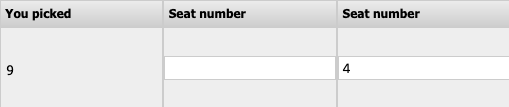
\includegraphics[width=\columnwidth]{figures/flight-booking.png}
  \caption{
    Graphical user interface generated from the specification in \cref{lst:flight-booking}.
    Three users are booking seats in parallel.
    The first user booked seat 9, the second did not enter a seat number yet, and the third is about to book seat 4.
  }
  \label{fig:flight-booking}
\end{figure}

With the returned list, we can state the predicate to verify the correctness of the booking process.
\setcounter{equation}{0}
\begin{align}
\psi(l)
   & =      \Len l \equiv 3 \label{flight-psi-exactly-three-seats}
\\ & \wedge \Uniq l \label{flight-psi-unique-seats}
\end{align}
The predicate specifies that all three passengers got exactly one seat (\ref{flight-psi-exactly-three-seats}), and that all seats are unique (\ref{flight-psi-unique-seats}), which means that no two passenger got the same seat.
The unary operators for list length ($\Len$) and uniqueness ($\Uniq$) are available in the predicate language.
List length is a capability of \SMTLIB, while $\Uniq$ is our own addition.
